\documentclass[11pt]{article}

\usepackage[margin=1in]{geometry}
\usepackage[T1]{fontenc}
\usepackage[utf8]{inputenc}
\usepackage[english]{babel}
\usepackage{lmodern}
\usepackage{microtype}
\usepackage{amsmath}
\usepackage{amssymb}
\usepackage{tabularx}
\usepackage{hyperref}
\usepackage{xcolor}
\usepackage{booktabs}
\usepackage{longtable}
\usepackage{array}
\usepackage{enumitem}
\usepackage{graphicx}
\usepackage{listings}
\usepackage{tikz}
\usetikzlibrary{arrows.meta, positioning, shapes.geometric, fit, calc, backgrounds}

\hypersetup{
  colorlinks=true,
  linkcolor=blue!50!black,
  urlcolor=blue!50!black,
  citecolor=blue!50!black,
  pdftitle={Technical Description of the ML2 Final Project},
  pdfauthor={GitHub Copilot}
}

\definecolor{codebg}{RGB}{247,247,247}
\definecolor{codeframe}{RGB}{220,220,220}

\lstdefinestyle{projectstyle}{
  basicstyle=\ttfamily\small,
  backgroundcolor=\color{codebg},
  frame=single,
  rulecolor=\color{codeframe},
  breaklines=true,
  columns=fullflexible,
  keepspaces=true,
  showstringspaces=false,
  tabsize=2
}

\lstset{style=projectstyle}

\newcommand{\pathtt}[1]{\texttt{#1}}

\title{Technical Description of the Project Architecture, Data Pipeline, and Training Workflow}
\author{ml2\_final\_project}
\date{\today}

\begin{document}

\maketitle

\begin{abstract}
This document explains the project at the level a new reader needs first: how the repository is organized, how the data moves from raw corpora to processed tensors, how the training code is split into reusable modules, and how the experiment folders are produced.

\end{abstract}

\tableofcontents
\newpage

\section{Proposal}
The goal of this project is to build a model for cross-ligual voice conversion. 
The model will be trained with the datasets: LibriSpeech-PT, TTS Portuguese Corpus, LibriSpeech-EN.
\section{Repository Overview}

The repository is divided into a few clear responsibilities: raw data storage, preprocessing, reusable code, experiment outputs, and documentation.

\subsection{High-Level Directory Tree}

\begin{lstlisting}
ml2_final_project/
|-- data/
|   |-- raw/
|   |   |-- libriSpeech-pt/
|   |   `-- tts-portuguese-Corpora/
|   |-- processed/
|   |   |-- libriSpeech-pt/
|   |   |   |-- train/
|   |   |   |   `-- librispeech_mels_metadata.csv
|   |   |   `-- test/
|   |   |       `-- librispeech_mels_metadata.csv
|   |   `-- tts_portuguese/
|   |       `-- mels_metadata.csv
|   |-- interim/
|   `-- external/
|-- scripts/
|   |-- download_datasets/
|   `-- preprocess/
|       |-- preprocess_libriSpeech-pt.py
|       `-- preprocess_mels_tts_portuguese.py
|-- src/
|   |-- data/
|   |   `-- first_step_data_loaders/
|   |       `-- datasets.py
|   |-- models/
|   |   `-- AcousticDecoder.py
|   |   `-- GST.py
|   |   `-- TextEncoder.py
|   |   `-- HiFi-GAN.py
|   `-- training/
|       `-- train_first_step/
|           |-- train.py
|           |-- model_loader.py
|           |-- losses.py
|           |-- train_utils.py
|           |-- text_processing.py
|           |-- configs.py
|           |-- run_training.py
|           `-- checkpoint_utils.py
|-- experiments/
|   `-- step_1/
|       `-- attempt_<timestamp>/
`-- docs/
\end{lstlisting}

\subsection{What Each Major Folder Means}

\begin{longtable}{>{\raggedright\arraybackslash}p{0.23\textwidth} >{\raggedright\arraybackslash}p{0.71\textwidth}}
\toprule
\textbf{Folder} & \textbf{Role in the project} \\
\midrule
\pathtt{data/raw} & Original corpora exactly as downloaded. Nothing here should depend on a model version or a feature extraction recipe. \\
\pathtt{data/processed} & Processed artifacts such as \pathtt{.pt} files and metadata CSV manifests used by the dataset layer. \\
\pathtt{data/interim} & Temporary intermediate outputs or scratch files that do not belong in the final processed dataset. \\
\pathtt{scripts/preprocess} & Reproducible preprocessing scripts that convert raw audio into filtered, normalized, indexed training samples. \\
\pathtt{src/data} & Dataset wrappers and batching helpers that turn manifests into PyTorch objects. \\
\pathtt{src/models} & Reusable neural network components. The architecture text in this document does not depend on these files as its source of truth. \\
\pathtt{src/training} & Training orchestration, losses, configuration presets, checkpointing, and experiment utilities. \\
\pathtt{experiments} & Timestamped or named experiment outputs. Each run keeps its config, checkpoints, logs, and TensorBoard data together. \\
\pathtt{docs} & Technical descriptions, reports, and the LaTeX sources for the project documentation. \\
\bottomrule
\end{longtable}

\section{End-to-End Data Flow}

The project follows a simple lifecycle:

\begin{enumerate}[leftmargin=1.5em]
  \item Download raw corpora into \pathtt{data/raw}.
  \item Preprocess audio and transcripts into standardized tensors.
  \item Save per-utterance artifacts and metadata manifests in \pathtt{data/processed}.
  \item Load the processed manifests with the dataset classes in \pathtt{src/data}.
  \item Build the training experiment from the modules in \pathtt{src/training}.
  \item Save checkpoints, logs, and plots under \pathtt{experiments/step\_1}.
\end{enumerate}

\subsection{Data Pipeline Diagram}

\begin{center}
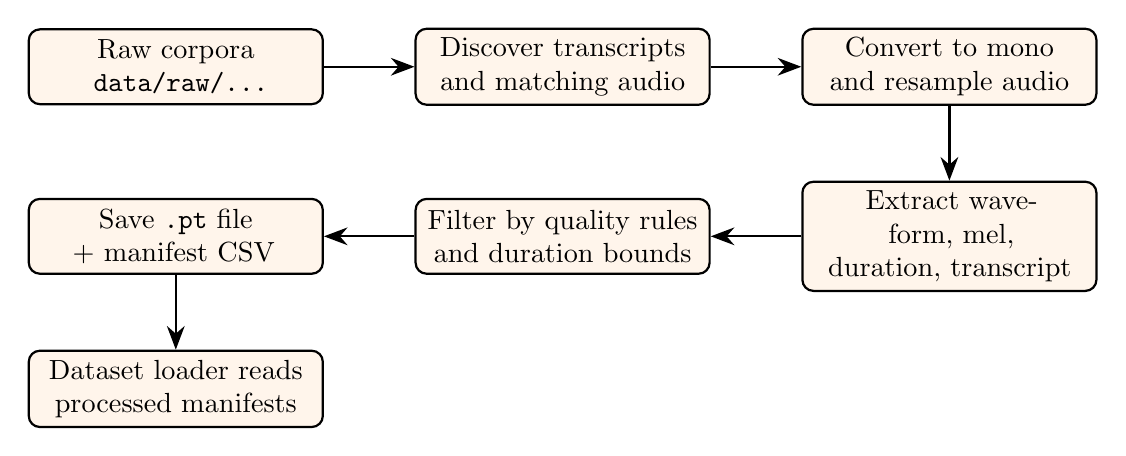
\begin{tikzpicture}[
  node distance=0.95cm and 1.15cm,
  block/.style={draw, rounded corners, thick, align=center, minimum height=0.95cm, text width=3.5cm, fill=orange!8},
  arrow/.style={-{Stealth[length=3mm]}, thick}
]
\node[block] (raw) {Raw corpora\\\pathtt{data/raw/...}};
\node[block, right=of raw] (discover) {Discover transcripts\\and matching audio};
\node[block, right=of discover] (normalize) {Convert to mono\\and resample audio};
\node[block, below=of normalize] (extract) {Extract waveform, mel,\\duration, transcript};
\node[block, left=of extract] (filter) {Filter by quality rules\\and duration bounds};
\node[block, left=of filter] (save) {Save \pathtt{.pt} file\\+ manifest CSV};
\node[block, below=of save] (load) {Dataset loader reads\\processed manifests};

\draw[arrow] (raw) -- (discover);
\draw[arrow] (discover) -- (normalize);
\draw[arrow] (normalize) -- (extract);
\draw[arrow] (extract) -- (filter);
\draw[arrow] (filter) -- (save);
\draw[arrow] (save) -- (load);
\end{tikzpicture}
\end{center}

\section{How Data Should Be Organized}

The project treats raw data and processed data as two different products. Raw data is the source of truth; processed data is a reusable training cache.

\subsection{Raw Data Layout}

Place each corpus in its own directory under \pathtt{data/raw}. A practical layout is:

\begin{lstlisting}
data/raw/
|-- libriSpeech-pt/
|   `-- mls_portuguese_opus/
|       |-- train/
|       |-- dev/
|       `-- test/
`-- tts-portuguese-Corpora/
    `-- TTS-Portuguese-Corpus/
        |-- audio/
        |-- text/
        `-- metadata/
\end{lstlisting}

The exact nested folder names may differ depending on how the corpus was downloaded, but the rule is the same: raw content stays grouped by dataset and is not overwritten by preprocessing.

\subsection{Processed Data Layout}

The processed area should mirror the dataset identity and the split that was used during preprocessing. The current project expects these main outputs:

\begin{lstlisting}
data/processed/
|-- libriSpeech-pt/
|   |-- train/
|   |   |-- <utt_id>.pt
|   |   `-- librispeech_mels_metadata.csv
|   `-- test/
|       |-- <utt_id>.pt
|       `-- librispeech_mels_metadata.csv
`-- tts_portuguese/
    |-- <utt_id>.pt
    `-- mels_metadata.csv
\end{lstlisting}

The dataset classes in \pathtt{src/data/first\_step\_data\_loaders/datasets.py} use these manifests directly. A sample CSV row can look like this:

\begin{lstlisting}[language=]
utt_id,text,duration,mel_path,audio_path
pt_000123,ola mundo,2.83,data/processed/libriSpeech-pt/train/pt_000123.pt,data/raw/libriSpeech-pt/.../pt_000123.flac
\end{lstlisting}

\subsection{What Goes Into a \pathtt{.pt} File}

Each serialized sample should keep everything needed to train or inspect the example later:

\begin{itemize}[leftmargin=1.5em]
  \item \pathtt{waveform}: the resampled mono waveform tensor.
  \item \pathtt{mel}: the log-mel spectrogram tensor, with 80 mel bins.
  \item \pathtt{sr}: the sample rate used by preprocessing, usually 22050 Hz.
  \item \pathtt{duration}: utterance duration in seconds.
  \item \pathtt{text}: the transcript text after normalization.
  \item \pathtt{utt\_id}: the unique utterance identifier.
  \item \pathtt{audio\_path}: the original audio path relative to the corpus root when available.
\end{itemize}

\subsection{Feature Extraction Parameters}

The preprocessing recipe is fixed so that every sample is compatible with the model input shape:

\begin{itemize}[leftmargin=1.5em]
  \item Sample rate: 22050 Hz.
  \item Mel bins: 80.
  \item FFT size: 1024.
  \item Window length: 1024.
  \item Hop length: 256.
  \item Mel frequency range: 0 Hz to 8000 Hz.
\end{itemize}

\subsection{Filtering Rules and Rationale}

A practical preprocessing pipeline should reject examples that are too short, too long, or malformed. In this project, the intended rule set is:

\begin{itemize}[leftmargin=1.5em]
  \item Minimum duration: 1.0 second.
  \item Maximum duration: 20.0 seconds.
  \item Mono waveform only.
  \item Resampled to the target sample rate.
  \item Transcript and audio must be aligned and non-empty.
\end{itemize}

These bounds keep padding under control, reduce memory spikes, and make batch shapes more predictable.

\section{Preprocessing Step by Step}

The preprocessing scripts in \pathtt{scripts/preprocess} are responsible for building the manifests used by training.

\subsection{Typical Workflow}

\begin{enumerate}[leftmargin=1.5em]
  \item Read the raw corpus root.
  \item Find transcript files and enumerate utterances.
  \item Match each transcript line to the corresponding audio file.
  \item Load audio with \pathtt{torchaudio}.
  \item Convert multichannel audio to mono if necessary.
  \item Resample to 22050 Hz.
  \item Compute the mel spectrogram with the fixed STFT configuration.
  \item Compute duration and apply the duration filter.
  \item Save the tensor payload to one \pathtt{.pt} file per utterance.
  \item Write the metadata CSV manifest.
  \item Optionally generate plots or sanity checks for a sample subset.
\end{enumerate}

\subsection{Example Preprocessing Command}

\begin{lstlisting}[language=bash]
python scripts/preprocess/preprocess_libriSpeech-pt.py \
  --input-dir data/raw/libriSpeech-pt/mls_portuguese_opus \
  --out-dir data/processed/libriSpeech-pt/train \
  --target-sr 22050 \
  --n-mels 80 \
  --n-fft 1024 \
  --hop-length 256 \
  --win-length 1024 \
  --min-duration 1.0 \
  --max-duration 10.0
\end{lstlisting}

\subsection{Why This Stage Matters}

This step is where the project becomes reproducible. If preprocessing is deterministic and documented, the same raw corpus always produces the same processed artifacts, and later training runs can be compared fairly.

\section{Dataset Loading and Batching}

The module \pathtt{src/data/first\_step\_data\_loaders/datasets.py} turns processed manifests into PyTorch datasets.

\subsection{Dataset Classes}

The current design uses three useful building blocks:

\begin{itemize}[leftmargin=1.5em]
  \item \pathtt{LibriSpeechPTDataset}: loads one LibriSpeech-PT split, typically \pathtt{train} or \pathtt{test}.
  \item \pathtt{TTSPortugueseDataset}: loads the TTS Portuguese processed manifest.
  \item \pathtt{CombinedFirstStepDataset}: concatenates multiple datasets into one training set.
\end{itemize}

\subsection{Default Training Mix}

The repository memory and dataset helpers agree on the default composition: LibriSpeech-PT train, LibriSpeech-PT test, and TTS Portuguese are combined for first-step training. That means the training code can treat the three sources as a single pool of processed examples.

\subsection{What Each Sample Returns}

Each dataset item returns a dictionary with the core information needed by the training loop:

\begin{itemize}[leftmargin=1.5em]
  \item \pathtt{mel}
  \item \pathtt{waveform}
  \item \pathtt{sr}
  \item \pathtt{duration}
  \item \pathtt{text}
  \item \pathtt{utt\_id}
  \item \pathtt{mel\_path}
  \item \pathtt{audio\_path}
  \item \pathtt{source}
\end{itemize}

\subsection{Batching Strategy}

Mel spectrograms and waveforms have variable lengths, so the collate function pads them along the time axis to the longest sample in the batch. The batch also keeps metadata such as the text string, utterance ID, duration, and source corpus name.

This is important for two reasons:

\begin{enumerate}[leftmargin=1.5em]
  \item Neural networks expect tensors with consistent batch dimensions.
  \item Metadata is needed for debugging and for later experiment analysis.
\end{enumerate}

\section{System Architecture: Train Structure}

The training phase is designed as a dual-pathway architecture processing both textual and acoustic features. The network maps Mel-spectrogram audio and corresponding text through cross-attention mechanisms, while simultaneously extracting stylistic features via a shared Global Style Token (GST) module.

\begin{center}
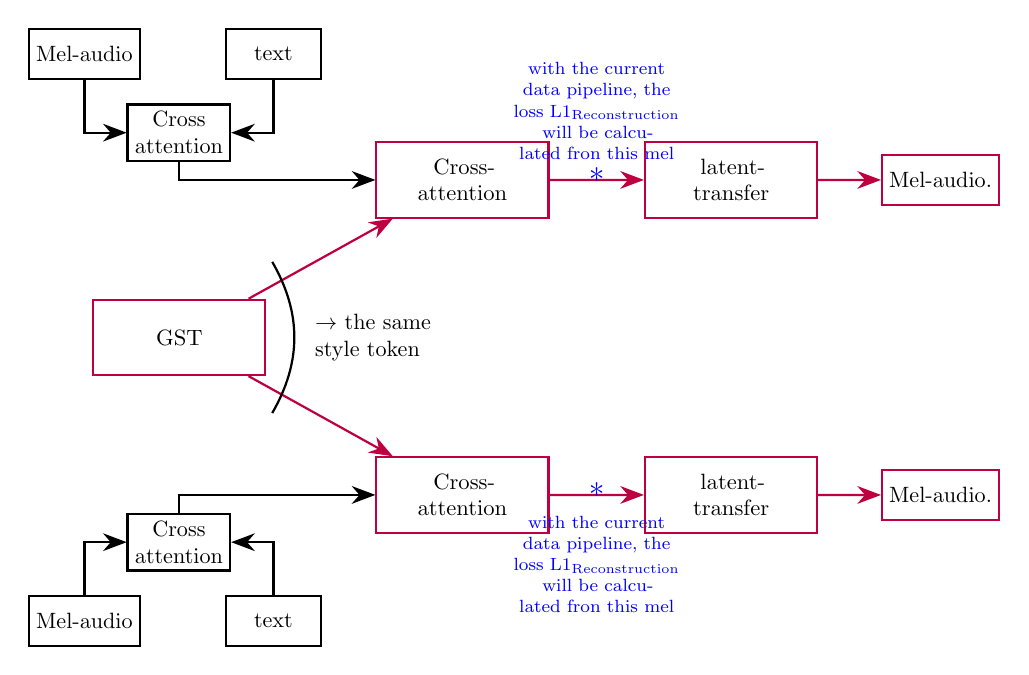
\begin{tikzpicture}[scale=0.8, transform shape,
  node distance=0.8cm and 1.2cm,
  block/.style={draw, rectangle, thick, minimum height=0.8cm, minimum width=1.5cm, align=center},
  largeblock/.style={draw, rectangle, thick, minimum height=1.2cm, minimum width=2.5cm, align=center, text width=2.5cm},
  arrow/.style={-{Stealth[length=3mm]}, thick}
]

% Middle branch (GST)
\node[largeblock, draw=purple] (gst) {GST};

% Top branch
\node[block] (mel_top) at (-1.5, 4.5) {Mel-audio};
\node[block] (text_top) at (1.5, 4.5) {text};
\node[block] (cross_small_top) at (0, 3.25) {Cross\\attention};
\draw[arrow] (mel_top) |- (cross_small_top);
\draw[arrow] (text_top) |- (cross_small_top);

\node[largeblock, draw=purple] (cross_large_top) at (4.5, 2.5) {Cross-\\attention};
\draw[arrow] (cross_small_top) |- (cross_large_top);
\draw[arrow, purple] (gst) -- (cross_large_top);

\node[largeblock, draw=purple, right=1.5cm of cross_large_top] (latent_top) {latent-\\transfer};
\draw[arrow, purple] (cross_large_top) -- node[above, font=\footnotesize, text=blue, text width=4cm, align=center, yshift=0.2cm] {with the current\\data pipeline, the loss L1\textsubscript{Reconstruction}\\will be calculated fron this mel} node[pos=0.5, font=\Large, text=blue] {*} (latent_top);

\node[block, draw=purple, right=1cm of latent_top] (mel_out_top) {Mel-audio.};
\draw[arrow, purple] (latent_top) -- (mel_out_top);

% Bottom branch
\node[block] (mel_bot) at (-1.5, -4.5) {Mel-audio};
\node[block] (text_bot) at (1.5, -4.5) {text};
\node[block] (cross_small_bot) at (0, -3.25) {Cross\\attention};
\draw[arrow] (mel_bot) |- (cross_small_bot);
\draw[arrow] (text_bot) |- (cross_small_bot);

\node[largeblock, draw=purple] (cross_large_bot) at (4.5, -2.5) {Cross-\\attention};
\draw[arrow] (cross_small_bot) |- (cross_large_bot);
\draw[arrow, purple] (gst) -- (cross_large_bot);

\node[largeblock, draw=purple, right=1.5cm of cross_large_bot] (latent_bot) {latent-\\transfer};
\draw[arrow, purple] (cross_large_bot) -- node[below, font=\footnotesize, text=blue, text width=4cm, align=center, yshift=-0.2cm] {with the current\\data pipeline, the loss L1\textsubscript{Reconstruction}\\will be calculated fron this mel} node[pos=0.5, font=\Large, text=blue] {*} (latent_bot);

\node[block, draw=purple, right=1cm of latent_bot] (mel_out_bot) {Mel-audio.};
\draw[arrow, purple] (latent_bot) -- (mel_out_bot);

% Bracket for Style Token annotation
\draw[thick] (gst.east) ++(0.1, 1.2) edge[bend left=30] node[right=0.2cm, align=left, text width=3cm] {$\rightarrow$ the same\\style token} ++(0, -2.4);

\end{tikzpicture}
\end{center}

\subsection{Pipeline Diagram}

\begin{center}
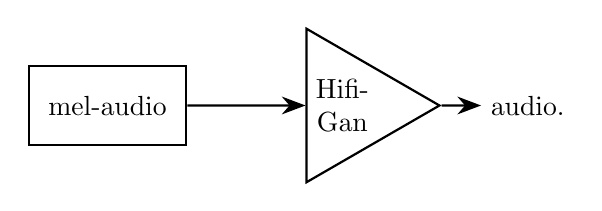
\begin{tikzpicture}[
  node distance=1.5cm,
  block/.style={draw, rectangle, thick, minimum height=1cm, minimum width=2cm, align=center},
  trapezoid/.style={draw, isosceles triangle, thick, isosceles triangle apex angle=60, shape border rotate=0, minimum height=1.5cm, align=center},
  arrow/.style={-{Stealth[length=3mm]}, thick}
]
\node[block] (mel) {mel-audio};
\node[trapezoid, right=of mel] (hifi) {Hifi-\\Gan};
\node[right=0.5cm of hifi] (audio) {audio.};

\draw[arrow] (mel) -- (hifi);
\draw[arrow] (hifi) -- (audio);
\end{tikzpicture}
\end{center}

During training, the central \pathtt{GST} module processes Mel-audio to output "the same style token," which is injected into both the top and bottom large \pathtt{Cross-attention} modules. The outputs pass through a \pathtt{latent-transfer} module before yielding the predicted \pathtt{Mel-audio}. Note that with the current data pipeline, the L1 Reconstruction loss will be explicitly calculated from the mel extracted at the marked ($*$) junction prior to latent-transfer.

\subsection{Vocoder Diagram}
For converting Mel-spectrograms back into waveform audio, a HiFi-GAN vocoder is utilized:

\vspace{0.5cm}
\begin{center}
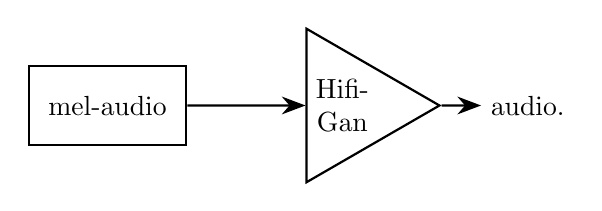
\begin{tikzpicture}[
  node distance=1.5cm,
  block/.style={draw, rectangle, thick, minimum height=1cm, minimum width=2cm, align=center},
  trapezoid/.style={draw, isosceles triangle, thick, isosceles triangle apex angle=60, shape border rotate=0, minimum height=1.5cm, align=center},
  arrow/.style={-{Stealth[length=3mm]}, thick}
]
\node[block] (mel) {mel-audio};
\node[trapezoid, right=of mel] (hifi) {Hifi-\\Gan};
\node[right=0.5cm of hifi] (audio) {audio.};

\draw[arrow] (mel) -- (hifi);
\draw[arrow] (hifi) -- (audio);
\end{tikzpicture}
\end{center}

\section{Loss Functions}

The loss objective combines multiple weighted criteria to govern perceptual quality, reconstruction accuracy across both languages, stylistic diversity, and emotional consistency. The complete formula is defined strictly as:

\[
\begin{aligned}
\text{Loss} = \;& \color{orange}w_1 \color{black}\text{Loss}_{\text{perceptual}}(\cdot) \\
& + \color{orange}w_2 \color{black} L1_{\text{Reconstruction}}(\text{predicted-Mel-inglish}, \text{target}) \\
& + \color{orange}w_2 \color{black} L1_{\text{Reconstruction}}(\text{predicted-Mel-Portuguese}, \text{target}) \\
& + \color{orange}w_3 \color{black} L_{\text{style-diversity}}(\text{all-the-style-tokens}) \\
& + \color{orange}w_4 \color{black} L_{\text{emotional-compatibility}}(\dots)
\end{aligned}
\]

\textbf{Implementation Notes:}
\begin{itemize}
    \item $\text{Loss}_{\text{perceptual}}$: Evaluated using the emotion classification network.
    \item $L_{\text{style-diversity}}$: Calculated based on the cosine similarity of all style tokens.
    \item $L_{\text{emotional-compatibility}}$: Currently undefined, but intended to utilize the classification network to assist in enforcing emotional consistency.
    \item Note that both reconstruction losses (English and Portuguese) share the same weight scalar $w_2$ in the standard formulation.
\end{itemize}

\section{Inference Workflow}

The inference stage describes how a translated language (English) is synthesized using audio from a source language (Portuguese). The network processes dual-language Mel audio and text, isolating the translated English features for output.

\textit{"For inference we will take a portuguese audio and output the inglish one. Ouor model is trained take: portuguese and english audio. So,"}

\subsection{Inference Architecture Diagram}

\begin{center}
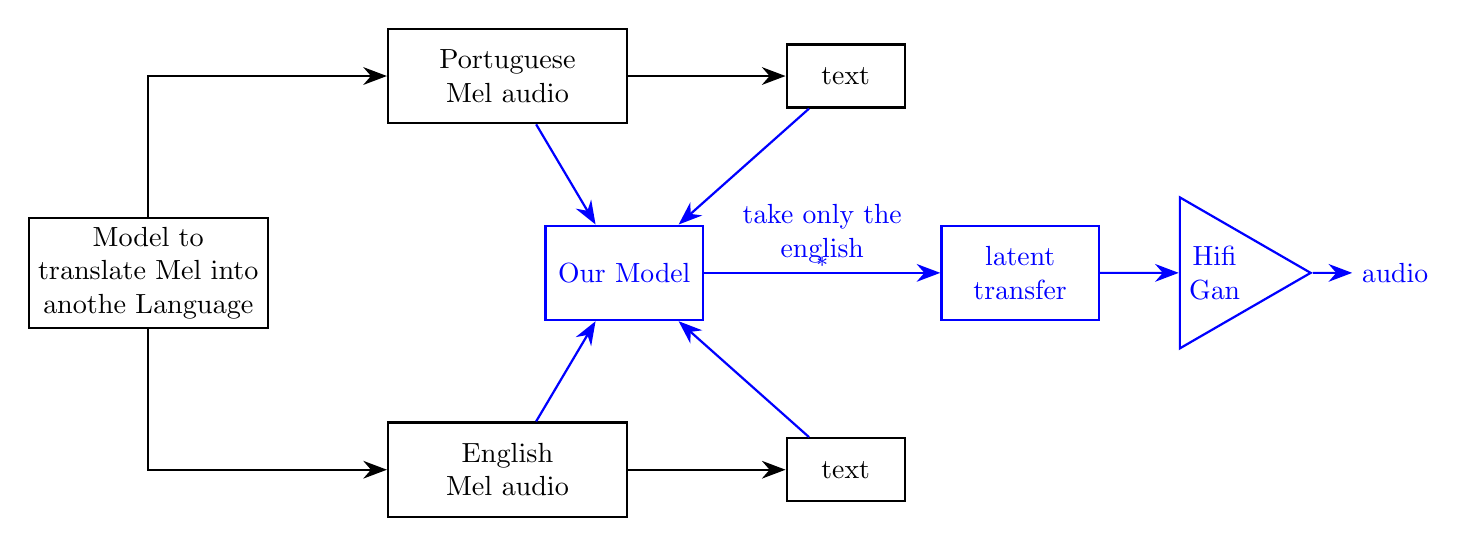
\begin{tikzpicture}[
  node distance=1.5cm and 2.0cm,
  block/.style={draw, rectangle, thick, minimum height=1.2cm, minimum width=2.5cm, align=center, text width=2.8cm},
  smallblock/.style={draw, rectangle, thick, minimum height=0.8cm, minimum width=1.5cm, align=center},
  modelblock/.style={draw, rectangle, thick, draw=blue, text=blue, minimum height=1.2cm, minimum width=2cm, align=center},
  trapezoid/.style={draw, isosceles triangle, thick, draw=blue, text=blue, isosceles triangle apex angle=60, shape border rotate=0, minimum height=1.5cm, align=center},
  arrow/.style={-{Stealth[length=3mm]}, thick},
  bluearrow/.style={-{Stealth[length=3mm]}, thick, blue}
]

\node[block] (translator) {Model to translate Mel into anothe Language};

\node[block, right=1.5cm of translator, yshift=2.5cm] (pt_mel) {Portuguese\\Mel audio};
\node[block, right=1.5cm of translator, yshift=-2.5cm] (en_mel) {English\\Mel audio};

\draw[arrow] (translator) |- (pt_mel);
\draw[arrow] (translator) |- (en_mel);

\node[smallblock, right=2cm of pt_mel] (text_pt) {text};
\node[smallblock, right=2cm of en_mel] (text_en) {text};

\draw[arrow] (pt_mel) -- (text_pt);
\draw[arrow] (en_mel) -- (text_en);

\node[modelblock, right=3.5cm of translator] (our_model) {Our Model};

\draw[bluearrow] (pt_mel) -- (our_model);
\draw[bluearrow] (en_mel) -- (our_model);
\draw[bluearrow] (text_pt) -- (our_model);
\draw[bluearrow] (text_en) -- (our_model);

\node[modelblock, right=3cm of our_model] (latent) {latent\\transfer};
\draw[bluearrow] (our_model) -- node[above, sloped, text=blue, align=center] {take only the\\english} node[pos=0.5, font=\footnotesize, text=blue, yshift=0.1cm] {*} (latent);

\node[trapezoid, right=1cm of latent] (hifi) {Hifi\\Gan};
\draw[bluearrow] (latent) -- (hifi);

\node[right=0.5cm of hifi, text=blue] (audio) {audio};
\draw[bluearrow] (hifi) -- (audio);

\end{tikzpicture}
\end{center}

\vspace{0.5cm}
\noindent \textit{* Maybe as a next step we can bail our own}


\begingroup\sloppy
The final model must receive only the Portuguese audio and output the English audio. 
For the first time, we will train only the model presented in the diagram arquetecture. 
The models for text-to-speech and speech-to-text are pre-trained. 

After having a good style token, we will try to build a model for text-to-speech and speech-to-text. 
\endgroup

\section{Training Code Organization in \pathtt{src}}

The training pipeline is split into small modules so that each concern has one main place in the codebase.

\subsection{Module Map}

\begin{longtable}{>{\raggedright\arraybackslash}p{0.23\textwidth} >{\raggedright\arraybackslash}p{0.71\textwidth}}
\toprule
\textbf{Module} & \textbf{What it does} \\
\midrule
\pathtt{train.py} & Main training entry point. Parses arguments, builds datasets, instantiates the model, runs training and validation, and writes outputs. \\
\pathtt{model\_loader.py} & Creates the full first-step TTS model from the submodules in \pathtt{src/models}. \\
\pathtt{losses.py} & Implements the objective terms used by training. \\
\pathtt{train\_utils.py} & Contains the epoch loops, checkpoint helpers, TensorBoard logging, and validation utilities. \\
\pathtt{text\_processing.py} & Converts transcript strings into token sequences. \\
\pathtt{configs.py} & Stores named training presets such as quick test, balanced, production, and lightweight runs. \\
\pathtt{run\_training.py} & Convenience launcher that selects a preset and forwards its arguments to \pathtt{train.py}. \\
\path{checkpoint_utils.py} & Utility commands for listing, comparing, and inspecting saved checkpoints. \\
\pathtt{test\_setup.py} & Sanity-check script for verifying that the environment and model loading work correctly. \\
\bottomrule
\end{longtable}

\subsection{Why This Modularization Helps}

Splitting the code this way makes the project easier to maintain and easier to review.

\begin{itemize}[leftmargin=1.5em]
  \item If a preprocessing bug appears, you only edit the scripts under \pathtt{scripts/preprocess}.
  \item If the model plan changes, you update the architecture description in this document and the corresponding training code together.
  \item If the loss definition changes, you touch \pathtt{losses.py} without rewriting the training loop.
  \item If you want a new experiment setup, you add a preset in \pathtt{configs.py} instead of duplicating a command by hand.
\end{itemize}

\subsection{Recommended Experiment Flow}

The practical order for a run is:

\begin{enumerate}[leftmargin=1.5em]
  \item Verify the environment with the setup test.
  \item Preprocess the raw corpora into \pathtt{data/processed}.
  \item Inspect one or two manifest rows and one or two \pathtt{.pt} files.
  \item Launch a small preset such as \pathtt{quick\_test}.
  \item Check the experiment directory and TensorBoard logs.
  \item Scale up to \pathtt{balanced} or \pathtt{production} after the pipeline is stable.
\end{enumerate}

\section{How to Run Experiments}

Experiments are stored in \pathtt{experiments/step\_1}. Every run creates a separate directory, usually named with a timestamp or a custom experiment name.

\subsection{Experiment Directory Tree}

\begin{lstlisting}
experiments/
`-- step_1/
    `-- attempt_YYYYMMDD_HHMMSS/
        |-- config.json
        |-- checkpoints/
        |   |-- epoch_0001.pt
        |   |-- epoch_0002.pt
        |   `-- best.pt
        |-- tensorboard/
        `-- logs/
\end{lstlisting}

\subsection{What Each Output Means}

\begin{itemize}[leftmargin=1.5em]
  \item \pathtt{config.json}: the exact hyperparameters used for the run.
  \item \pathtt{checkpoints/}: saved training states that allow resuming or evaluating later.
  \item \pathtt{tensorboard/}: event files for loss curves, metrics, and qualitative logs.
  \item \pathtt{logs/}: human-readable training logs or auxiliary text output.
\end{itemize}

\subsection{Example Commands}

\begin{lstlisting}[language=bash]
# Quick smoke test
python src/training/train_first_step/run_training.py quick_test

# Balanced default run
python src/training/train_first_step/run_training.py balanced

# Full custom training
python src/training/train_first_step/train.py \
  --num-epochs 100 \
  --batch-size 32 \
  --learning-rate 1e-3 \
  --weight-reconstruction 1.0 \
  --weight-diversity 0.5 \
  --acoustic-decoder-hidden-size 256 \
  --acoustic-decoder-num-layers 3 \
  --style-embedding-dim 128 \
  --num-workers 4 \
  --experiment-name cross_lingual_training
\end{lstlisting}

\subsection{Monitoring a Run}

You can monitor training with TensorBoard:

\begin{lstlisting}[language=bash]
tensorboard --logdir experiments/step_1/<experiment_name>/tensorboard
\end{lstlisting}

Useful curves include total loss, reconstruction loss, diversity loss, validation metrics, and any audio examples logged from the vocoder.

\section{Step-by-Step Guide from Download to Training}

This section is the shortest path from a fresh corpus to a reproducible model run.

\subsection{1. Download the datasets}

Place the raw archives in \pathtt{data/raw}. Do not preprocess before the download tree is complete.

\subsection{2. Verify the folder structure}

Make sure the corpus layout is readable by the preprocessing scripts. If a dataset uses different folder names, adapt the input path before running the script.

\subsection{3. Run preprocessing}

Use the scripts in \pathtt{scripts/preprocess} to create the processed dataset. The result should be one \pathtt{.pt} file per utterance plus a manifest CSV.

\subsection{4. Inspect a few outputs}

Open one manifest row and one saved sample to confirm that the mel tensor, waveform, duration, and transcript look sane.

\subsection{5. Confirm the dataset loader can read the manifests}

The dataset module should successfully resolve the \pathtt{mel\_path} entries and return dictionaries with consistent keys.

\subsection{6. Start with a small experiment}

Run \pathtt{quick\_test} first. It is designed for a fast sanity check, not for final quality.

\subsection{7. Scale up}

After the small run works, move to \pathtt{balanced} or a custom training command.

\subsection{8. Review the experiment artifacts}

Check \pathtt{config.json}, the best checkpoint, the TensorBoard curves, and any generated audio logs.

\section{How to Modularize the Project Cleanly}

If you want to extend the project without creating a monolithic script, keep each responsibility in the same layer where it already belongs.

\subsection{Adding a New Dataset}

Add a new preprocessing script under \pathtt{scripts/preprocess}, write the processed files under \path{data/processed/<new_dataset>}, and create a matching dataset wrapper under \path{src/data/first_step_data_loaders}.

\subsection{Adding a New Model Component}

Create the neural module in \pathtt{src/models}, then wire it into the implementation layer that uses the conceptual architecture described above. If the component changes the loss behavior, update \pathtt{losses.py} at the same time.

\subsection{Adding a New Experiment Variant}

Put the hyperparameters in \pathtt{configs.py}. That keeps command-line invocations short and makes experiments easy to reproduce.

\subsection{Adding Better Debugging}

Log examples, shapes, and checkpoints from \pathtt{train\_utils.py}. Keep debug output next to the training loop, not scattered across unrelated modules.

\section{Practical Example of the Whole Workflow}

A complete minimal run might look like this:

\begin{enumerate}[leftmargin=1.5em]
  \item Download LibriSpeech-PT and TTS Portuguese into \pathtt{data/raw}.
  \item Preprocess both corpora and write manifests into \pathtt{data/processed}.
  \item Launch \pathtt{python src/training/train\_first\_step/run\_training.py quick\_test}.
  \item Confirm that checkpoints are created under \pathtt{experiments/step\_1}.
  \item Open TensorBoard and check that losses decrease as expected.
  \item If everything is stable, rerun with the balanced preset.
\end{enumerate}

\section{Summary}

The project is organized around a simple engineering rule: raw data stays in \pathtt{data/raw}, processed artifacts stay in \pathtt{data/processed}, reusable code lives in \pathtt{src}, and experiment outputs live in \pathtt{experiments}. The model architecture in this document is diagram-driven, not code-driven. That keeps the explanation aligned with the conceptual design the project is trying to communicate.

\end{document}
